\documentclass{sigchi}

% Use this command to override the default ACM copyright statement (e.g. for preprints). 
% Consult the conference website for the camera-ready copyright statement.


%% EXAMPLE BEGIN -- HOW TO OVERRIDE THE DEFAULT COPYRIGHT STRIP -- (July 22, 2013 - Paul Baumann)
% \toappear{Permission to make digital or hard copies of all or part of this work for personal or classroom use is 	granted without fee provided that copies are not made or distributed for profit or commercial advantage and that copies bear this notice and the full citation on the first page. Copyrights for components of this work owned by others than ACM must be honored. Abstracting with credit is permitted. To copy otherwise, or republish, to post on servers or to redistribute to lists, requires prior specific permission and/or a fee. Request permissions from permissions@acm.org. \\
% {\emph{CHI'14}}, April 26--May 1, 2014, Toronto, Canada. \\
% Copyright \copyright~2014 ACM ISBN/14/04...\$15.00. \\
% DOI string from ACM form confirmation}
%% EXAMPLE END -- HOW TO OVERRIDE THE DEFAULT COPYRIGHT STRIP -- (July 22, 2013 - Paul Baumann)


% Arabic page numbers for submission. 
% Remove this line to eliminate page numbers for the camera ready copy
% \pagenumbering{arabic}


% Load basic packages
\usepackage{balance}  % to better equalize the last page
\usepackage{graphics} % for EPS, load graphicx instead
\usepackage{times}    % comment if you want LaTeX's default font
\usepackage{url}      % llt: nicely formatted URLs
\usepackage{array}

\usepackage{booktabs}
\newcommand{\ra}[1]{\renewcommand{\arraystretch}{#1}}

% llt: Define a global style for URLs, rather that the default one
\makeatletter
\def\url@leostyle{%
  \@ifundefined{selectfont}{\def\UrlFont{\sf}}{\def\UrlFont{\small\bf\ttfamily}}}
\makeatother
\urlstyle{leo}


% To make various LaTeX processors do the right thing with page size.
\def\pprw{8.5in}
\def\pprh{11in}
\special{papersize=\pprw,\pprh}
\setlength{\paperwidth}{\pprw}
\setlength{\paperheight}{\pprh}
\setlength{\pdfpagewidth}{\pprw}
\setlength{\pdfpageheight}{\pprh}

% Make sure hyperref comes last of your loaded packages, 
% to give it a fighting chance of not being over-written, 
% since its job is to redefine many LaTeX commands.
\usepackage[pdftex]{hyperref}
\hypersetup{
pdftitle={SIGCHI Conference Proceedings Format},
pdfauthor={LaTeX},
pdfkeywords={SIGCHI, proceedings, archival format},
bookmarksnumbered,
pdfstartview={FitH},
colorlinks,
citecolor=black,
filecolor=black,
linkcolor=black,
urlcolor=black,
breaklinks=true,
}

% create a shortcut to typeset table headings
\newcommand\tabhead[1]{\small\textbf{#1}}


% End of preamble. Here it comes the document.
\begin{document}

\title{Kinesiological Control of Teleoperated \\Robotic Manipulators}

\numberofauthors{3}
\author{
  \alignauthor Christopher Bodden\\
    \affaddr{University of Wisconsin-Madison}\\
    \affaddr{1210 W. Dayton St.\\ Madison, WI 53706}\\
    \email{cbodden@cs.wisc.edu}
  \alignauthor Danny Rakita\\
    \affaddr{University of Wisconsin-Madison}\\
    \affaddr{1210 W. Dayton St.\\ Madison, WI 53706}\\
    \email{rakita@cs.wisc.edu}
  \alignauthor Alper Sarikaya\\
    \affaddr{University of Wisconsin-Madison}\\
    \affaddr{1210 W. Dayton St.\\ Madison, WI 53706}\\
    \email{sarikaya@cs.wisc.edu}
}

\maketitle

\begin{abstract}
While robots have the potential for increasing dexterity for completing manufacturing tasks, the lack of naturalistic robot manipulation make it difficult for non-experts to control the robot for a desired task. We explore the question of naturalistic control of a robot arm for tasks that have one-to-one mapping to natural human movement, and those that do not against typical joystick control. Through our exploration, we have developed a system that uses computer vision and a data glove to determine an individual's hand position and orientation in three-dimensional space. We map this position and orientation input to the robot's end effector. We show that using a combination of kinesiological control plus specialty functions can achieve similar performance and user perceptions to a joystick. Additionally, kinesiological control without direct mapping to the full range of the robot's actuated motion impairs performance for tasks that could benefit from it. Interestingly, task type had a strong effect on user perception of the control method. We note that further research in this area is needed to fully explore the potential of kinesiological control of co-working robots.
\end{abstract}

\keywords{
  Robot manipulation, naturalistic control, user study
}

\category{H.5.m.}{Information Interfaces and Presentation (e.g. HCI)}{Miscellaneous}

\section{Introduction}

Manipulation of external robot interfaces can be a challenging task, and moreso to enable novice controllers to control actuated motion with dexterity.  The multitude of methods and techniques for manipulating many robot actuators to accomplish seemingly simple tasks generally require extensive training and practice.  Many typical control methods for actuated robots require the operator to make a cognitive map from control space to the three-dimensional space in which the robot operates.  In our work, we explore kinesological control of a robot arm for novice users, looking at precision tasks that have a one-to-one mapping with human motion and those that do not.  We construct this kinesological control with conventional joystick manipulation, which provides more direct input to the robot.  

In the implementation of our work, we have developed a system that uses computer vision to track an individual's arm in three-dimensional space and map that input to the end effector of a Kinova Mico robot arm.  Our kinesological implementation allows for real-time manipulation and control of the robot arm in real-time, and in conjunction with gyroscope readings from a smart glove worn by the individual, allows a user to move, rotate, and actuate fingers of the hand without direct manipulation of a joystick (see Figure~\ref{fig:demo} for sample setup). In our experimentation, we also allow users to use the Kinova-included joystick to accomplish similar tasks. Through our study, we show how tasks that do not map one-to-one with natural movement can have limitations that need non-kinesological (e.g. direct) control to overcome.  However, we also show that depending on the task type, the control type had a strong effect on user perception.

\begin{figure}[t]
	\centering
	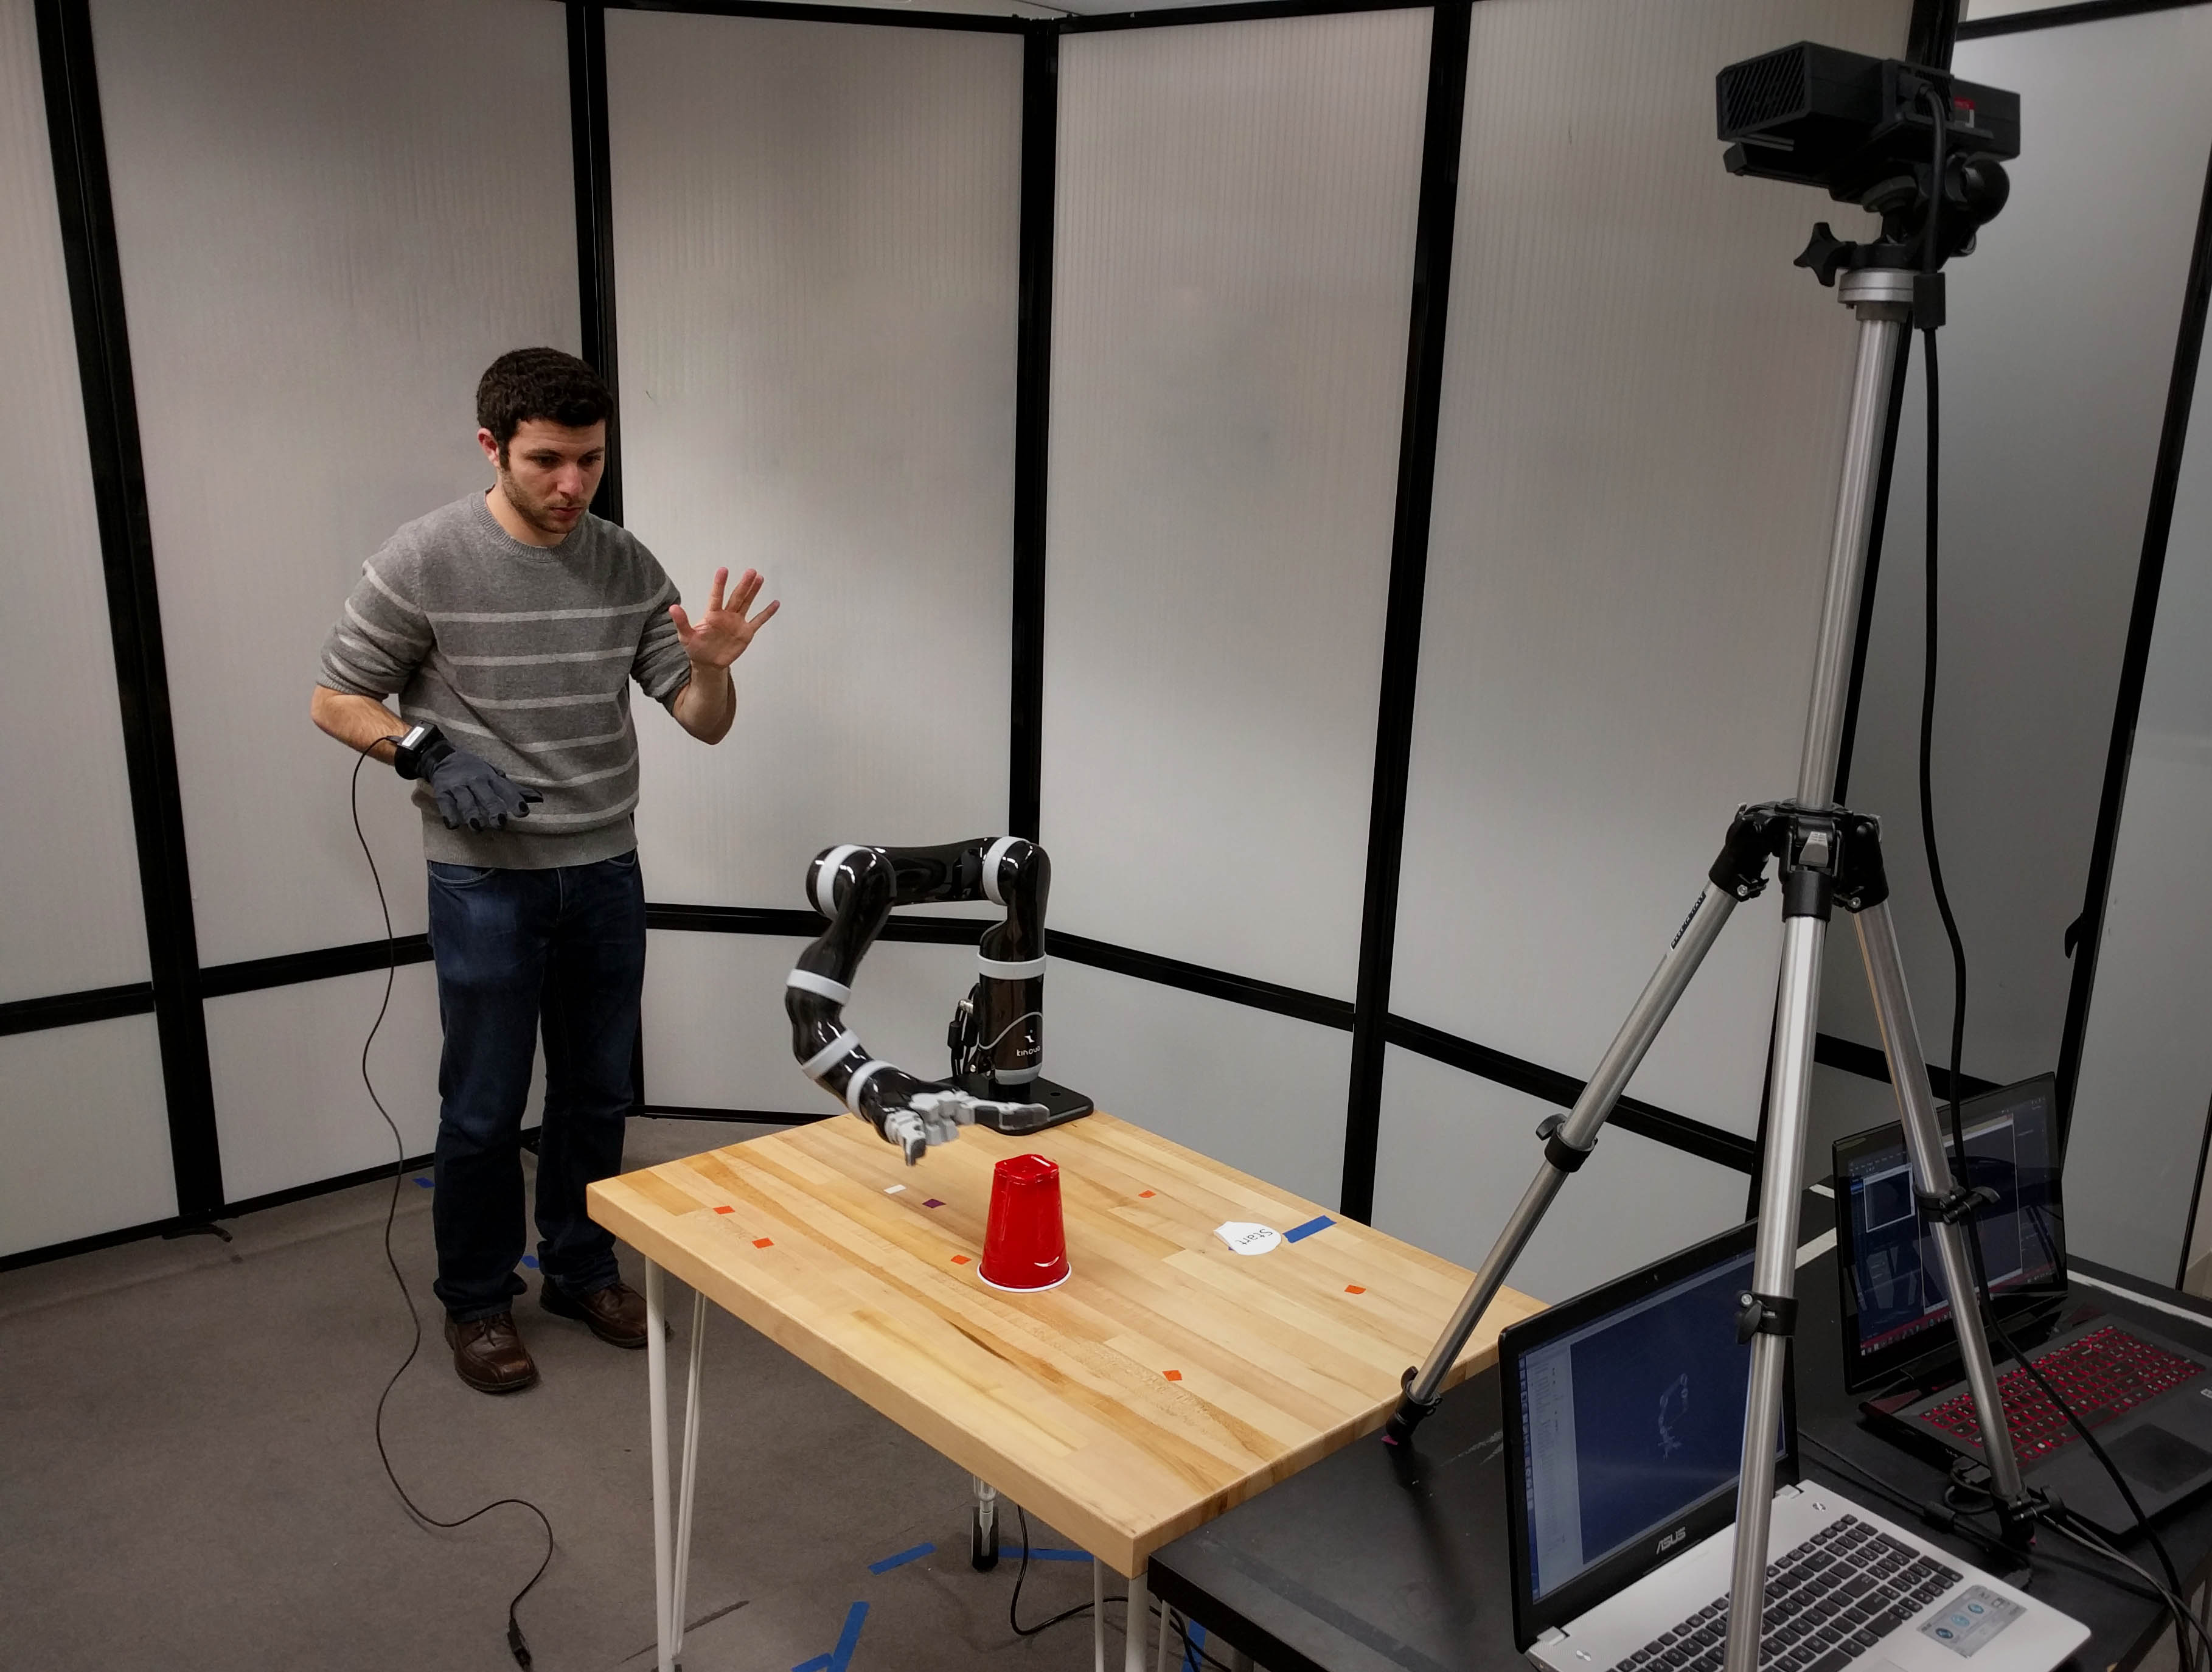
\includegraphics[width=\columnwidth]{../Data/Figures/kinesiological_demo_2.jpg}
	\caption{The context of our model experiment.  The Kinect is on the tripod with a clear view of the participant and his right arm, while a data glove captures hand orientation.  The participant is motioning with his off-hand for the robot to open its gripper.}
	 \label{fig:demo}
\end{figure} 

\section{Background}

Advances in the areas of computer vision and robot control have enabled us to rapidly prototype and use these techniques to allow for novice control of a robot arm.  In particular, we utilized the Kinect for Windows SDK~\cite{Kinect} to quickly capture an individual's arm with a Microsoft Kinect.  By piping hand locations over the network to a machine running ROS (Robot Operating System) ~\cite{ROS} interfaced to the Kinova robot arm, we are able to directly control the robot using kinesiological control.

Several prior studies have looked at how remote control of robots can assist in manufacturing and human-robot collaboration tasks. Our work context follows a long line of research in bilateral teleoperation (see Hokayem and Spong for a wide-spanning survey~\cite{hokayem2006bilateral}), which concerns issues of stability and telepresence.  Critically, the two-way feedback mechanisms between the human operator and the robotic analog needs to be such to minimize perceptible latency in the connection, and also provide enough feedback to judge and adapt input.  Park \emph{et al.}~\cite{park2003robust} represents some early work in teleoperation to help smooth error in input to the robot's output trajectory.  
% The authors use differing stiffnesses of objects that the robot interacts with to vary how the robot communicates with the controller, and represents an advancement in bilateral teleoperation.

In more recent work, research has started to generalize insights from individual application of telepresence applications.  In particular, Dragan \emph{et al.}~\cite{dragan2013teleoperation} explore teleoperation with customizable interfaces.  Importantly, they identify that both the task context and assistive scaffolding (e.g. input goal estimation) are necessary to support teleoperation and manipulations of complex systems. Specific to the goals of our project, Gi-Hun \emph{et al.}'s work on online retargeting for teleoperation~\cite{yang2013online} shows the utility of using the Kinect to collect natural movement of an operator and mapping input to the end-effector of a robot, while Labonte \emph{et al.}~\cite{labonte2010comparative} identify potential scaffolds to assist novice users using different viewpoints in telehomecare applications.  While this work sets the context for our work, no work to date has looked at supporting and empirically evaluating different kinesthetic methods for novice control of an actuated robot.

In constructing our qualitative scales for post-hoc questionnaires, we used two seminal studies to report user preferences.  Davis~\cite{Davis1989} presents a methodological approach to measuring participants' perceived usefulness, ease-of-use, and acceptance of information interfaces. Although we adapt this to robot-human interaction, this adaptation of this scale to other interfaces has some precedence---Lin \emph{et al.}~\cite{Lin2008} uses such an adaptation to measure interaction and perception of experience on the Internet.  
% We use the scale to measure user perceived usefulness, ease-of-use, and acceptance of the control method with regard to each task performed.

\section{Experimental Study}

Our study involved different control methods of a Kinova Mico arm, while looking at different types of tasks that either do or do not map easily to natural human movement.  
% In order to enable capture of participants arm motion to manipulate the robot arm, w
We use the Kinect to capture the position of the participant's right hand in three-dimensional space, and use a VML data glove to capture fine-grained hand orientation.  The participant has the ability to use their off-hand to change the gripper state on the robot arm---a closed fist and an open palm close and open the gripper, respectively.  Input is captured on one machine and passes along hand position, orientation, and gripper state via UDP packets at 4Hz to a receiving machine running the ROS application that commands the Mico robot arm. 
% Figure~\ref{fig:demo} shows an example setup of an experimental trial. 

Our research question concerns the effect of kinesiological robot arm control on novice user task performance and perception for tasks that do or do not have kinesiological mappings to human motion.  Based on our two tasks, we derived three input modalities, two of which are based on our kinesiological capture system.  One modality captures the hand position and orientation, while the other augments this with direct control of non-natural robot actuation (e.g. rotating the robot wrist more than a full rotation).  We call this second modality ``kines+'' in our work. The third input control is the Mico robot's included joystick.  The joystick has several modes---the primary moves the end effector in three-dimensional space through a bidirectional pad and twists of the control knob.  The other modes modify elbow orientation or wrist orientation and hand gripping.  

\subsection{Study Design}

We designed a $3\times2$ mixed-methods design with the three input modalities: joystick, kinesiological control, and kinesiological augmented with direct input (kines+); and two task types: direct mapping to natural movement, and robot-augmented movement.  We implemented our study as a mixed-methods design to minimize learning effects of manipulating the robot. Control modality was between-participants and task type was within-participants. Each participant was randomly assigned a control modality and asked to complete two tasks (in counterbalanced order).

\subsection{Hypotheses}

\textbf{H1:} We hypothesize that kinesiological control of the robot arm for natural mappings of tasks will perform better than the two other modes of control, and likewise hypothesize that direct control of the robot with the joystick will help users accomplish tasks that do not have direct mappings. Furthermore, we hypothesize that the combined control method (kines+) will perform as well or better than kinesiological control for tasks with natural mappings, and as well or better than joystick control for tasks without natural mappings.

\textbf{H2:} We hypothesize that the same relationships as \textbf{H1} will hold for our participant perceptions, (ease-of-use, usefulness, and enjoyment) of the control method as well. We believe this because kinesiological control should feel more natural and easier to control for tasks with direct mappings, while the additional range of motion provided by the joystick should be perceived better on tasks with no direct mapping. 
% [alper: this seems kind of redundant with the above]
% Kines+ provides the best of this two conditions, so we believe it will perform as well or better than the other conditions.

% \textbf{[set up study, what components we used, the task types, the experimental design, stats about the participant]}

\subsection{Participants \& Procedure}

We recruited participants ($n=12$) from within a university setting between the ages of 19--40 ($\mu=27.1, \sigma=5.5$; 2 females, 10 males). Participants received a candy bar as compensation for and all completed the study within 10 minutes. 
% The total study time per a participants was 10 minutes.

Participants were randomly assigned their input modality randomly.  Each participant was given an instruction sheet with how to manipulate the robot and given an unbounded amount of time to manipulate and practice with the assigned input method.  Once confirmation was given by the participant to proceed, they were given an instruction sheet for the task.  After confirming that no clarification questions were needed, a timer was started and stopped when the desired action was completed, with an upper-bound of five minutes.  The one-to-one mapping task requested the participant to move a cup from one location on a table to another location (we call this the ``movement'' task), while the non one-to-one mapping required a 360$^{\circ}$ rotation of the cup in-place (requiring lifting of the cup; ``rotation'' task).  Upon completion, the remaining task type was administered in the same fashion.  After the completion of the two tasks, demographic and robot familiarity information was collected. Each participant completed each task for their randomly assigned input modality once. 

\subsection{Measures}

\begin{table}[t]
\centering
\ra{1.2}
\begin{tabular}{@{}l@{}}
\toprule
\em{Ease of Use} ($\alpha = 0.81$) \\
1) The control method made it easy to accomplish the task. \\
2) I felt confident controlling the robot. \\
3) I could accurately control the robot. \\
\midrule
\em{Usefulness} ($\alpha = 0.74$) \\
1) Controlling the robot was easy to understand. \\
2) I would like to control a robot like this in the future. \\
3) I found the control method useful. \\
\midrule
\em{Enjoyment} ($\alpha = 0.85$) \\
1) Controlling the robot was fun. \\
2) I felt satisfied while controlling the robot. \\
3) I felt happy while controlling the robot. \\
\bottomrule
\end{tabular}
\caption{Subjective questions asked after each trial for task type for each participant. \label{tab:subjective}}
\end{table}


To evaluate participants' performance, we measured one objective metric, \textit{score}, by normalizing the time taken to complete each task by the time allotment of five minutes.

To measure participants' perception of different control types for each task type, we administered a questionnaire, inspired by scales proposed by Davis and Lin~\cite{Davis1989, Lin2008}, after each unique combinations of factors measuring participant perception of the manipulation method with the task type along dimensions of \textit{usefulness}, \textit{ease-of-use}, and \textit{enjoyment}. Three questions per measure were asked along each of the subjective dimensions, shown in Table \ref{tab:subjective}, using a seven-point rating scale from strongly disagree (1) to strongly agree (7). Cronbach's $\alpha$ was $\geq0.7$ for each dimension, confirming the reliability of each scale. Factor analysis was also performed. Three factors were above the Kaiser criterion, and within these factors the loadings for each question were grouped as described in the table.

% \textbf{[what measures we did, how we split up the participants, the procedure that each participant saw]}

\subsection{Results}

Participants data was analyzed for each measure using full-factorial analysis of variance (ANOVA). For each measure, control type was modeled as between participants and task type was modeled as within participants. Pairwise comparisons were made using Tukey HSD Post Hoc tests. Our analysis also includes equivalence analysis, where our threshold for equivalence is $p\geq0.25$. Our hypotheses are concerning interaction effects between control type and task type; however, main effects from independent variables are also reported here. Results are shown in Figure \ref{fig:bar_chart}.

\begin{figure}[t]
	\centering
	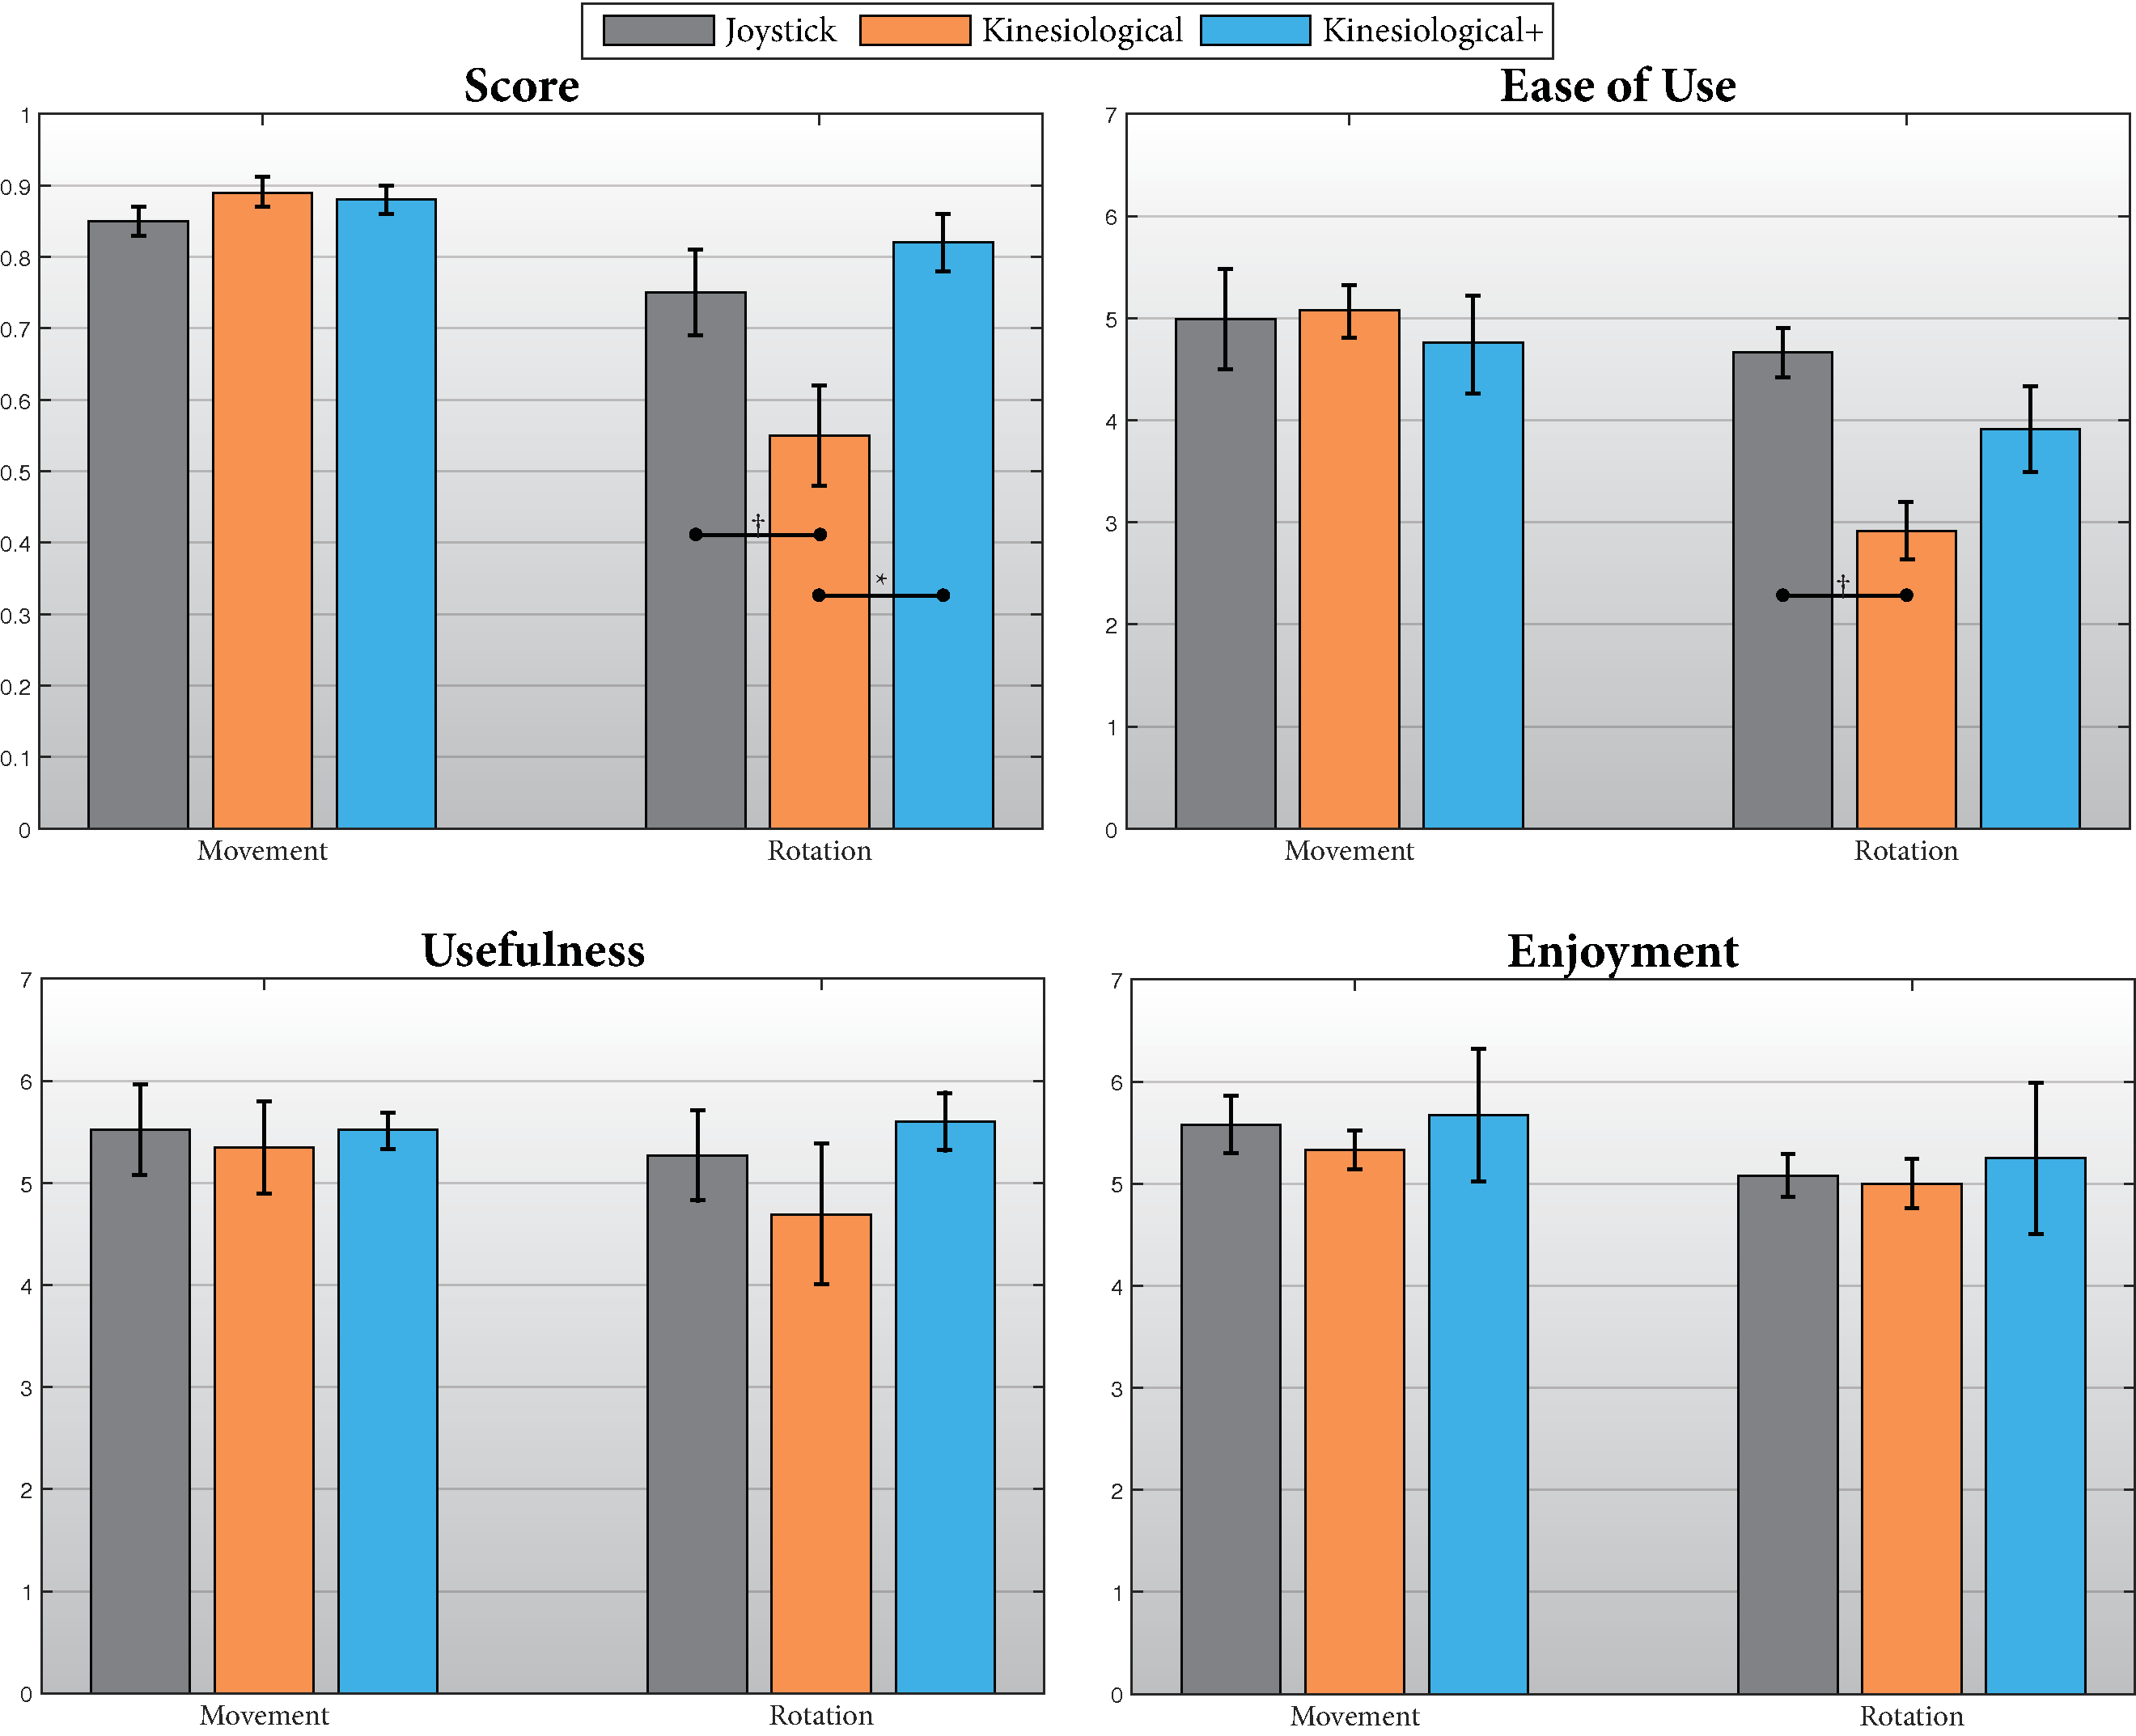
\includegraphics[width=\columnwidth]{figures/bar_charts.pdf}
	\caption{Results objective (top-left) and subjective measures. Kinesiological control impairs user performance and perceived ease of use for the rotation (no 1-to-1 mapping) task. However, there is no difference between joystick and kines+ control. \em{Error bars represent standard error.} $\ast: p \leq 0.01, \dagger:p \leq 0.05 $ }
	\label{fig:bar_chart}
\end{figure} 

\subsubsection{Task performance}

Participants scored ($R^{2}=0.79$) higher (took less time to complete the tasks) using \textit{kines+} control ($M=0.85$, $SD=0.06$) than \textit{joystick} control ($M=0.80$, $SD=0.10$). \textit{Joystick} control likewise scored higher than \textit{kinesiological} control ($M=0.72$, $SD=0.20$). Control type had a marginal main effect on score ($F(2, 9)=3.94, p=0.06$). Pairwise comparisons showed a significant difference between control types \textit{kines+} and \textit{kinesiological} ($p=0.05$). Score was found to be equivalent for control types \textit{kines+} and \textit{joystick} ($p=0.55$). Participants scored higher on the \textit{movement} task ($M=0.87$, $SD=0.04$) than on the \textit{rotation} task ($M=0.71$, $SD=0.15$). Task type was a significant main effect on score ($F(1, 9)=28.6, p<0.001$).

The interaction of control type and task type was also significant ($F(2, 9)=7.62, p=0.01$). Participants scored higher using \textit{kines+} control ($M=0.82$, $SD=0.07$) than \textit{kinesiological} control ($M=0.55$, $SD=0.13$) for the \textit{rotation} task type. Likewise,  participants scored higher using \textit{joystick} control ($M=0.75$, $SD=0.12$) than \textit{kinesiological} control for the \textit{rotation} task type. Both of these interaction were significant effects on score (\textit{joystick}-\textit{kinesiological}: $p=0.04$; \textit{kines+}-\textit{kinesiological}: $p=0.003$). 
There were significant effects between task types and control types, but not relevant in our analysis.
% All other significant interaction were across task types, which is not relevant to our hypotheses.

\subsubsection{User perception}

Participants rated ease of use ($R^{2}=0.65$) for the \textit{movement} task ($M=4.94$, $SD=0.78$) higher than the \textit{rotation} task ($M=3.83$, $SD=0.95$). The main effect of task type was significant on ease of use ($F(1, 9)=14.6, p=0.004$). The interaction of control type$\times$task type marginally affected ease of use ($F(2, 9)=3.55, p=0.07$). Specifically, the \textit{kinesiological}-\textit{joystick} pair for the \textit{rotation} task was a significant effect on ease of use ($p=0.04$). Participants rated ease of use higher for \textit{joystick} control ($M=4.67$, $SD=0.47$) than \textit{kinesiological} control ($M=2.92$, $SD=0.57$) for the \textit{rotation} task type. 
% All other significant interaction were across task types, which is not relevant to our hypotheses. 
The interaction of the \textit{kines+} and \textit{joystick} control type pair for both task types appears to come from the same population (\textit{rotation}: $p=0.72$; \textit{movement}: $p=1.00$). Perceived ease of use was not significantly affected by control type ($F(2, 9)=2.28, p=0.16$).

Perceived usefulness ($R^{2}=0.84$) was not significantly affected by control type ($F(2, 9)=0.47, p=0.64$), task type ($F(1, 9)=1.90, p=0.20$), or the interaction of control type$\times$task type  ($F(2, 9)=1.16, p=0.36$). 
% It's worth noting that the interation of the \textit{kines+}-\textit{joystick} control type pair for both task types appears to come from the same population (\textit{rotation}: $p=0.99$; \textit{movement}: $p=1.00$).
However, equivalence testing between \textit{kines+} and \textit{joystick} control for both task types seem to come from the same population (\textit{rotation}: $p=0.99$; \textit{movement}: $p=1.00$).

Participants rated enjoyment ($R^{2}=0.89$) for the \textit{movement} task ($M=5.53$, $SD=0.78$) higher than the \textit{rotation} task ($M=5.11$, $SD=0.84$). The main effect of task type was significant on enjoyment ($F(1, 9)=6.08, p=0.04$). Participant enjoyment was not significantly affected by control type ($F(2, 9)=0.12, p=0.89$) or the interaction of control type and task type  ($F(2, 9)=0.08, p=0.92$). The interation of the \textit{kines+} and \textit{joystick} control pair for both task types appears to come from the same population (\textit{rotation}: $p=1.00$; \textit{movement}: $p=1.00$).

\subsection{Discussion}

Our results were able to provide some support for \textbf{H1}. Performance for kines+ is similar to kinesiological control for direct mapping tasks and similar to joystick control for tasks with no direct mapping. Joystick control outperforms kinesiological control for tasks with no direct mapping. However, contrary to \textbf{H1}, kinesiological control was not significantly better performing versus joystick control for our "movement" task.% direct mapping tasks.

Our results provide limited support for \textbf{H2} as perceptions of kines+ is similar to kinesiological control for direct mapping tasks and similar to joystick control for tasks with no direct mapping. However, the hypothesized perception difference between joystick and kinesiological was only apparent for ease of use in the no direct mapping task. We hypothesize several factors could contribute to the lack of significant results. First our sample size is small ($n=12$). Second, we believe for many novice robot users, the novelty of controlling the robot is perceived well even when performance is impaired.

\section{Future Work \& Conclusion}
This work explored the use of kinesiological control of robot arms as an alternative to traditional joystick and knob controls. We explored control types with respect to two task modalities. While we lacked stastical power to provide evidence for our entire hypotheses, we did show that kinesiological control performs as well as and is perceived similarly to traditional joystick control if the kinesiological control is combined with special abilities provided by the robot. We believe this finding is important to guide improved kinesiological control designs. Designers should consider additional abilities afforded by the robot when implementing retargetting and provide these abilities to the user.

In the future we would like to perform our study with more participants, as well as more trials for each task per participant. We believe this would increase the power of our findings and help to differentiate between control types. We would also like to explore more advanced retargetting, as our work presented here only accounted for the end-effector of the robot. More advanced retargetting could allow manipulation of the position and orientation of each robot link to match the user's demonstration. This improvement could potentially improve how natural kinesiological control feels to novice users.

% \begin{table}
  % \centering
  % \begin{tabular}{|c|c|c|}
    % \hline
    % \tabhead{Objects} &
    % \multicolumn{1}{|p{0.3\columnwidth}|}{\centering\tabhead{Caption --- pre-2002}} &
    % \multicolumn{1}{|p{0.4\columnwidth}|}{\centering\tabhead{Caption --- 2003 and afterwards}} \\
    % \hline
    % Tables & Above & Below \\
    % \hline
    % Figures & Below & Below \\
    % \hline
  % \end{tabular}
  % \caption{Table captions should be placed below the table.}
  % \label{tab:table1}
% \end{table}

\section{Acknowledgments}

We thank Professor Bilge Multu and Michael Gleicher for discussions in designing the user study, and also thank our participants for their in-depth comments and enthusiasm for the system.  
% The authors are supported by a number of different grants (ha!).

% Balancing columns in a ref list is a bit of a pain because you
% either use a hack like flushend or balance, or manually insert
% a column break.  http://www.tex.ac.uk/cgi-bin/texfaq2html?label=balance
% multicols doesn't work because we're already in two-column mode,
% and flushend isn't awesome, so I choose balance.  See this
% for more info: http://cs.brown.edu/system/software/latex/doc/balance.pdf
%
% Note that in a perfect world balance wants to be in the first
% column of the last page.
%
% If balance doesn't work for you, you can remove that and
% hard-code a column break into the bbl file right before you
% submit:
%
% http://stackoverflow.com/questions/2149854/how-to-manually-equalize-columns-
% in-an-ieee-paper-if-using-bibtex
%
% Or, just remove \balance and give up on balancing the last page.
%
\balance

\bibliographystyle{acm-sigchi}
\bibliography{robot-control}
\end{document}
